% Please use the skeleton file you have received in the
% invitation-to-submit email, where your data are already
% filled in. Otherwise please make sure you insert your
% data according to the instructions in PoSauthmanual.pdf
%\documentclass[article]
%{jpconf}
\documentclass[a4paper]{jpconf}
\usepackage{graphicx}
\usepackage{epstopdf} 
\begin{document}

\title{Liquid Argon optical properties to be used in Geant4 and Opticks Simulations}

\author{ Hans~Wenzel$^1$}

\address{ $^1$~Fermilab PO Box 500, Batavia, IL 60510,
USA}

\ead{wenzel@fnal.gov}

\begin{abstract}
  In Geant4 and Opticks optical properties like e.g. the refractive
  index, absorption length, rayleigh scattering length etc. as well as surface properties are inputs that have to be provided.
  In this paper we collect the
  optical properties relevant for liquid Argon TPC's.   
\end{abstract}
%\tableofcontents
\section{Introduction}
  In Geant4 and Opticks optical properties like e.g. the materials refractive
  index are inputs that have to be provided when the detector is constructed.  High-precision modeling of 
  light production, transport and detection in liquid Argon  experiments requires the use of the best available values to describe the properties of liquid Argon.
In this article we briefly
  describe the physical processes relevant to the production, transport and detection of optical photons in liquid Argon.
  We collect the
  values and parameterizations of optical properties relevant for liquid Argon TPC's. We provide scripts that plot this quantities and that convert this values
  into a gdml description that can be directly used in the Geant4 Detector description.
  All values are summarized in the file material.xml which can be found in the github repository \cite{ref:scripts}.
  Usually quantities are given as a function of photon wavelength but Geant4 requires the photon energy.
  The motion of the charged particles liberates
charge from the surrounding argon (ionization) and
produces light (scintillation)



\begin{equation}
  E_{\gamma}(eV) = \frac{h  c}{\lambda_{\gamma} \times  10^{-9}}
  \label{equ:equation1}
\end{equation}
\noindent
    with:\\
  speed of light: $c = 299792458 m/sec$\\
  Planck constant: $h = 4.13566743\times10^{-15} eV/sec$\\
  \clearpage
  \section{Light production}
  There are two relevant sources of light production when a charged particle passes through a medium. The two sources have very different characteristics and yield. One is Scintillation light produced when a
  charged particle ionizes the material. The light is emitted isotropic from the point where it is produced. 
  

  
  Cerenkov radiation (\cite{ref:pdg},\cite{ref:wikipedia}) is electromagnetic radiation emitted when a charged particle passes through a dielectric medium at a speed greater than the phase velocity
  (speed of propagation of a wavefront in a medium) of light in that medium.
  Cerenkov radiation as conical wave front with the emission angle given by 
   \begin{equation}
  \cos \theta ={\frac {1}{n\beta }}
   \end{equation}
  with:\\
   ratio between the speed of the particle $v_p$ and the speed of light as $\beta =\frac{v_p}{c}$.


  \subsection{Scintillation Properties of liquid Argon}

  Efficient scintillator with typical Light yields in the order of a few 10,000’s of photons per $MeV$  deposited (depends on E field, particle type and purity)
  (SCINTILLATIONYIELD: $50000/MeV$ when no electric field present)
Scintillation yield is E-field and particle
dependent. For a proton:
24,000 photons / MeV, E = 500 V / cm
40,000 photons / MeV, E = 0 V / cm
  
  Liquid argon produces scintillation light via two distinct scintillation mechanisms, each
  of which has a different characteristic time constant. The emission spectra are passed to Geant4
  as a 2 column matrix where the first column is the photon energy and the second is the value.

  \begin{table}[h!]
  \begin{center}
    \label{tab:table1}
    \begin{tabular}{|l|l|c|} % <-- Alignments: 1st column left, 2nd middle and 3rd right, with vertical lines in between
      \hline
      \textbf{Property}& \textbf{Geant4 keyword}\footnote{The Geant4 keywords used in this article refer to Geant4 version $ > 11.0$ released in December 2021. The latest version introduced changes to the Geant4 API with regards to optical material properties.}  &       \textbf{value}\\
      \hline
      light yield&SCINTILLATIONYIELD & $50000 \gamma 's/MeV$ (no electric field)\\
      Wavelength of emission&SCINTILLATIONCOMPONENT1 &  $128nm$ ($FWHM=10nm$) see \ref{fig:spectrum}\\
      Wavelength of emission&SCINTILLATIONCOMPONENT2 &  $128nm$ ($FWHM=10nm$)  see \ref{fig:spectrum}\\
      fast component&SCINTILLATIONTIMECONSTANT1& $6 ns$\\  
      fast fraction&SCINTILLATIONYIELD1& $0.75$ \\
      slow component&SCINTILLATIONTIMECONSTANT2& $1500 ns$ \\
      slow fraction&SCINTILLATIONYIELD2& $0.25$\\
                   &RESOLUTIONSCALE& $1$\\
      \hline
    \end{tabular}
  \end{center}
  \caption{Scintillation Properties of liquid Argon.}
  \end{table}

  Scintillation Quenching,
  Birks law below:
\begin{equation}
  \frac {dL}{dx}=S\frac {\frac {dE}{dx}}{1+kB{\frac {dE}{dx}}}.
  \label{equ:birks}
\end{equation}
  where L is the light yield, S is the scintillation efficiency, dE/dx is the specific energy loss of the particle per path length,  kB is the Birks coefficient. Its value depends on the scintillating material.
\begin{figure}
\centering
\begin{minipage}{.5\textwidth}
  \centering
  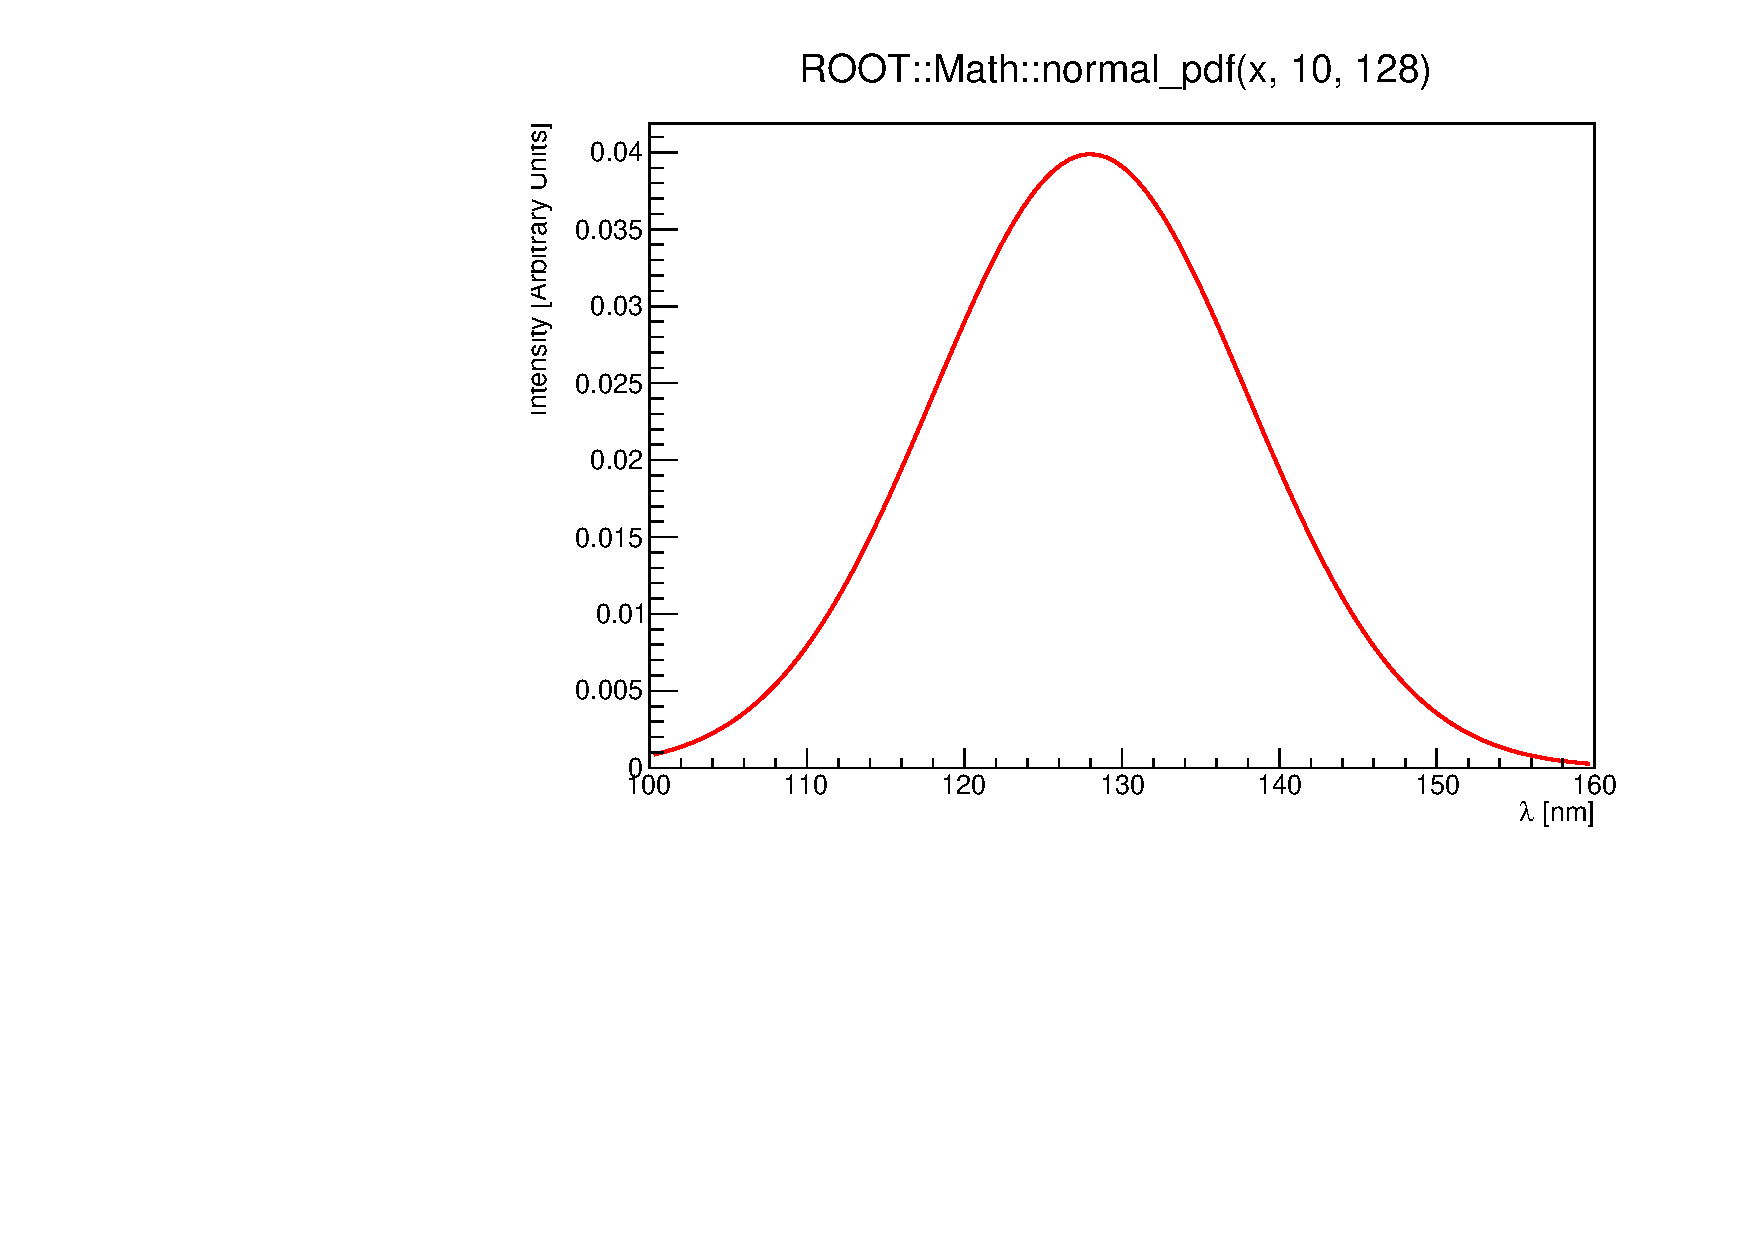
\includegraphics[width=.7\linewidth]{spectrum.pdf}
%  \captionof{figure}{A figure}
%  \label{fig:spectrum}
\end{minipage}%
\begin{minipage}{.5\textwidth}
  \centering
  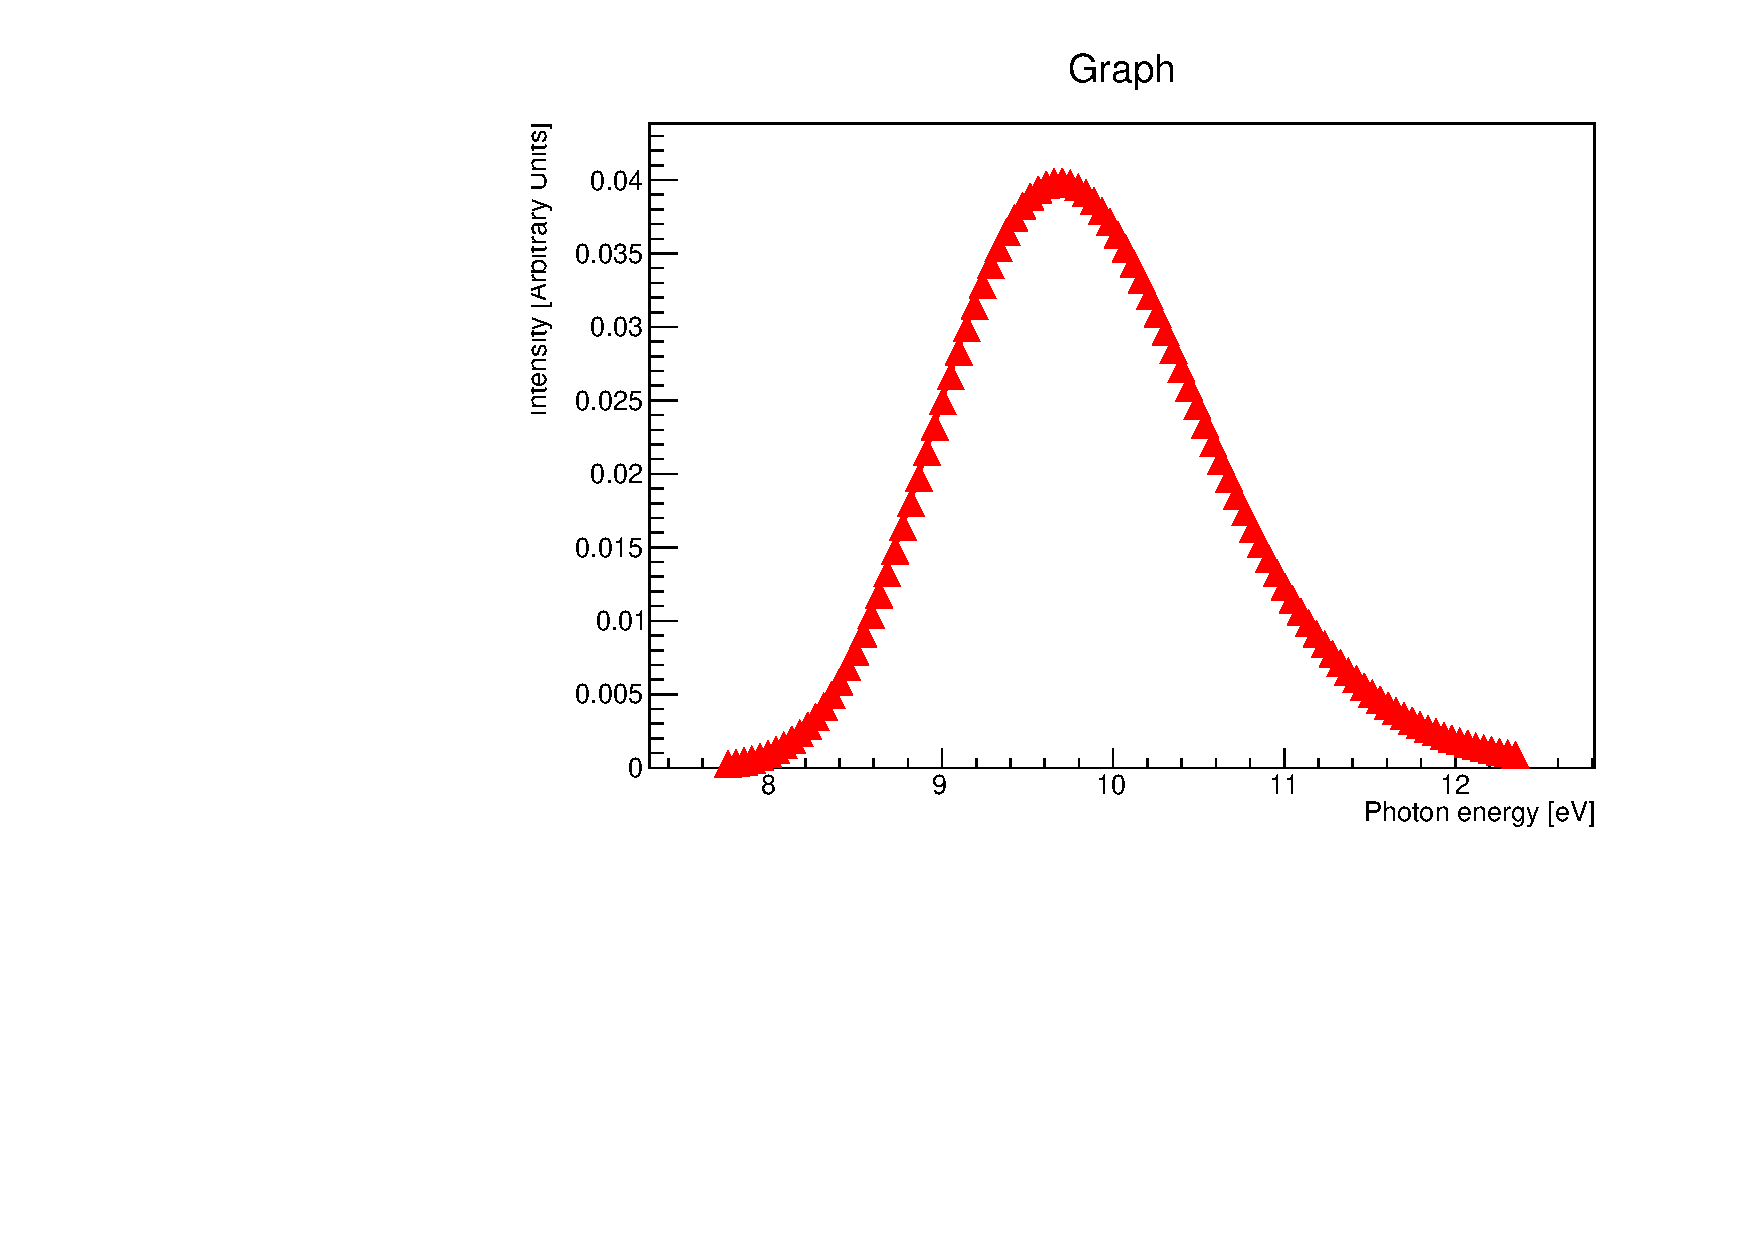
\includegraphics[width=.7\linewidth]{spectrumE.pdf}
%  \captionof{figure}{Another figure}
%  \label{fig:spectrumE}
\end{minipage}
\caption{\label{fig:spectrum}Scintillation emission spectrum.}
\end{figure}

\subsection{Cerenkov spectrum and Yield}
A charged particle radiates if its speed is greater than the local phase speed of light $v_p$. 
In Geant4 the process is not contributing to energy loss.

the charged particle travels in a medium with speed $v_p$  such that
$\frac{c}{n} < v_p < c$.
from \cite{ref:pdg}
\begin{equation}
  \cos(\theta_C)= \frac{1}{n \beta}
  \label{equ:ceren1}
\end{equation}
\begin{equation}
  \frac{d^2N}{dEdx} = \frac{2 \pi \alpha  z^2}  {\lambda^2} \left(1 - \frac{1}{(\beta^2 n^2(\lambda))}\right)
  \label{equ:ceren2}
\end{equation}
\begin{figure}[ht]
\begin{center}
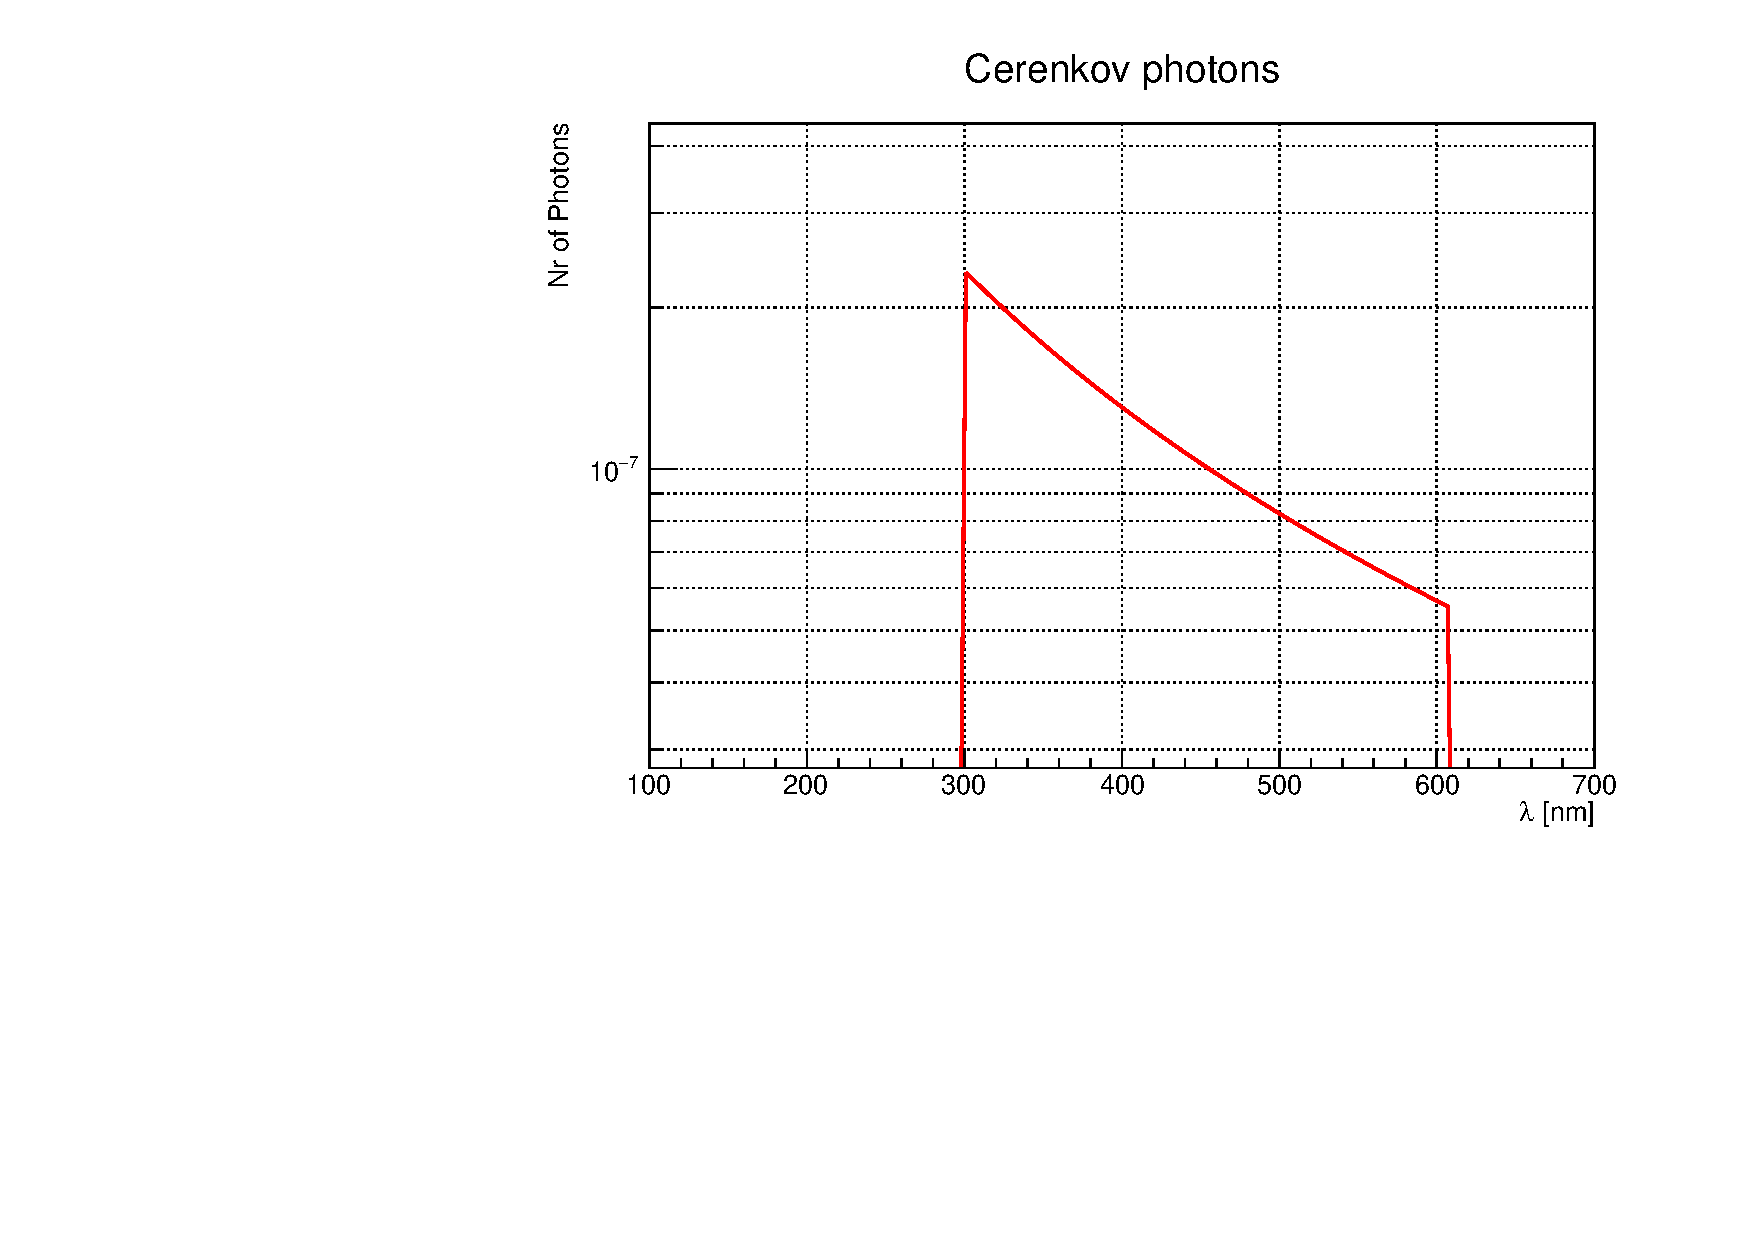
\includegraphics[width=35.5pc]{cerenkov.pdf}
\end{center}
\caption{\label{fig:cerenkov}Cerenkov spectrum}
\end{figure}

\clearpage
\section{Light propagation}
In this section we discuss the material properties related to light propagation in a medium. The values are 
passed to Geant4 as a 2 column matrix where the first column is the photon energy and the second is the value. 
 
\begin{table}[h!]
  \begin{center}
    \label{tab:table1}
    \begin{tabular}{|c|c|} 
      \hline
      \textbf{optical material property} & \textbf{Geant4 Keyword}\\
      \hline
      Refraction index as function of photon energy &RINDEX      \\
      Absorption length as function of photon energy& ABSLENGTH   \\
      Rayleigh scattering length as function of photon energy & RAYLEIGH    \\
      \hline
    \end{tabular}
  \end{center}
  \caption{Material properties related to light propagation in a medium}
 \end{table}

\subsection{Refraction Index and group velocity}

In \cite{ref:vg} the refraction index and group velocity  at $128 nm$ are measured at $n = 1.358 \pm 0.003$ and $\frac{1}{vg} = 7.46 \pm 0.08 ns/m$.
( compared to $n= 1.45 \pm 0.07$ \cite{ref:grace})

$\frac{1}{vg} = 7.46 \pm 0.08 ns/m$ corresponds to $0.134 m/nsec$ which is approximately $c_0/2240$ where $c_0$ is the speed of light in vacuum.
(reading it from the gdml dump calculated by Geant4 one gets $c_0/2600$)



The Sellmeier equation \ref{equ:sellmeier} below is an empirical relationship between refractive index and wavelength for a particular transparent medium.
\begin{equation}
n^2 = a_0 + \frac{a_{UV} \lambda^2}{\lambda^2 -\lambda^2_{UV}}+\frac{a_{IR}\lambda^2}{\lambda^2 - \lambda^2_{IR}}.
 \label{equ:sellmeier}
\end{equation}

 \begin{table}[h!]
  \begin{center}
    \label{tab:table1}
    \begin{tabular}{|c|c|c|} 
      \hline
      \textbf{ Scintillation $\lambda$} &\textbf{UV Resonance $\lambda_{UV}$} &\textbf{IR Resonance $\lambda_{IR}$}\\
 (nm)           & (nm)          &(nm) \\
      \hline
128 & 106.6 &908.3\\
      \hline
    \end{tabular}
  \end{center}
  \caption{blabla bla.}
 \end{table}
 
 \begin{table}[h!]
  \begin{center}
    \label{tab:table1}
    \begin{tabular}{|c|c|c|c|} 
      \hline
\textbf{ $T (K) $}& \textbf{ $a_0$} & \textbf{ $a_{UV}$} & \textbf{ $a_{IR}$ }\\
\hline
      $83.81$ & $1.24\pm0.09$ & $0.27\pm0.09$ & $0.00047\pm0.007$ \\
$90$ & $1.26\pm 0.09$& $0.23\pm 0.09$ & $0.0023\pm0.007$ \\
      \hline
    \end{tabular}
  \end{center}
  \caption{Sellmeier coefficients}
 \end{table}
 
where the parameters $a_0$ , $a_{UV}$ and $a_{IR}$ known as Sellmeier coefficients have to be determined
experimentally.
 
 The relation between group velocity and the refraction index is given by:

\begin{equation}
  v_g (\lambda)= \frac{c}{n-\lambda \frac{\partial{n}}{\partial{\lambda}}}
      \label{equ:vgroup}
% \caption{relation between refraction index and group velocity.}       
\end{equation}

 


% \caption{relation between refraction index and group velocity.} 
\begin{figure}[ht]
\begin{center}
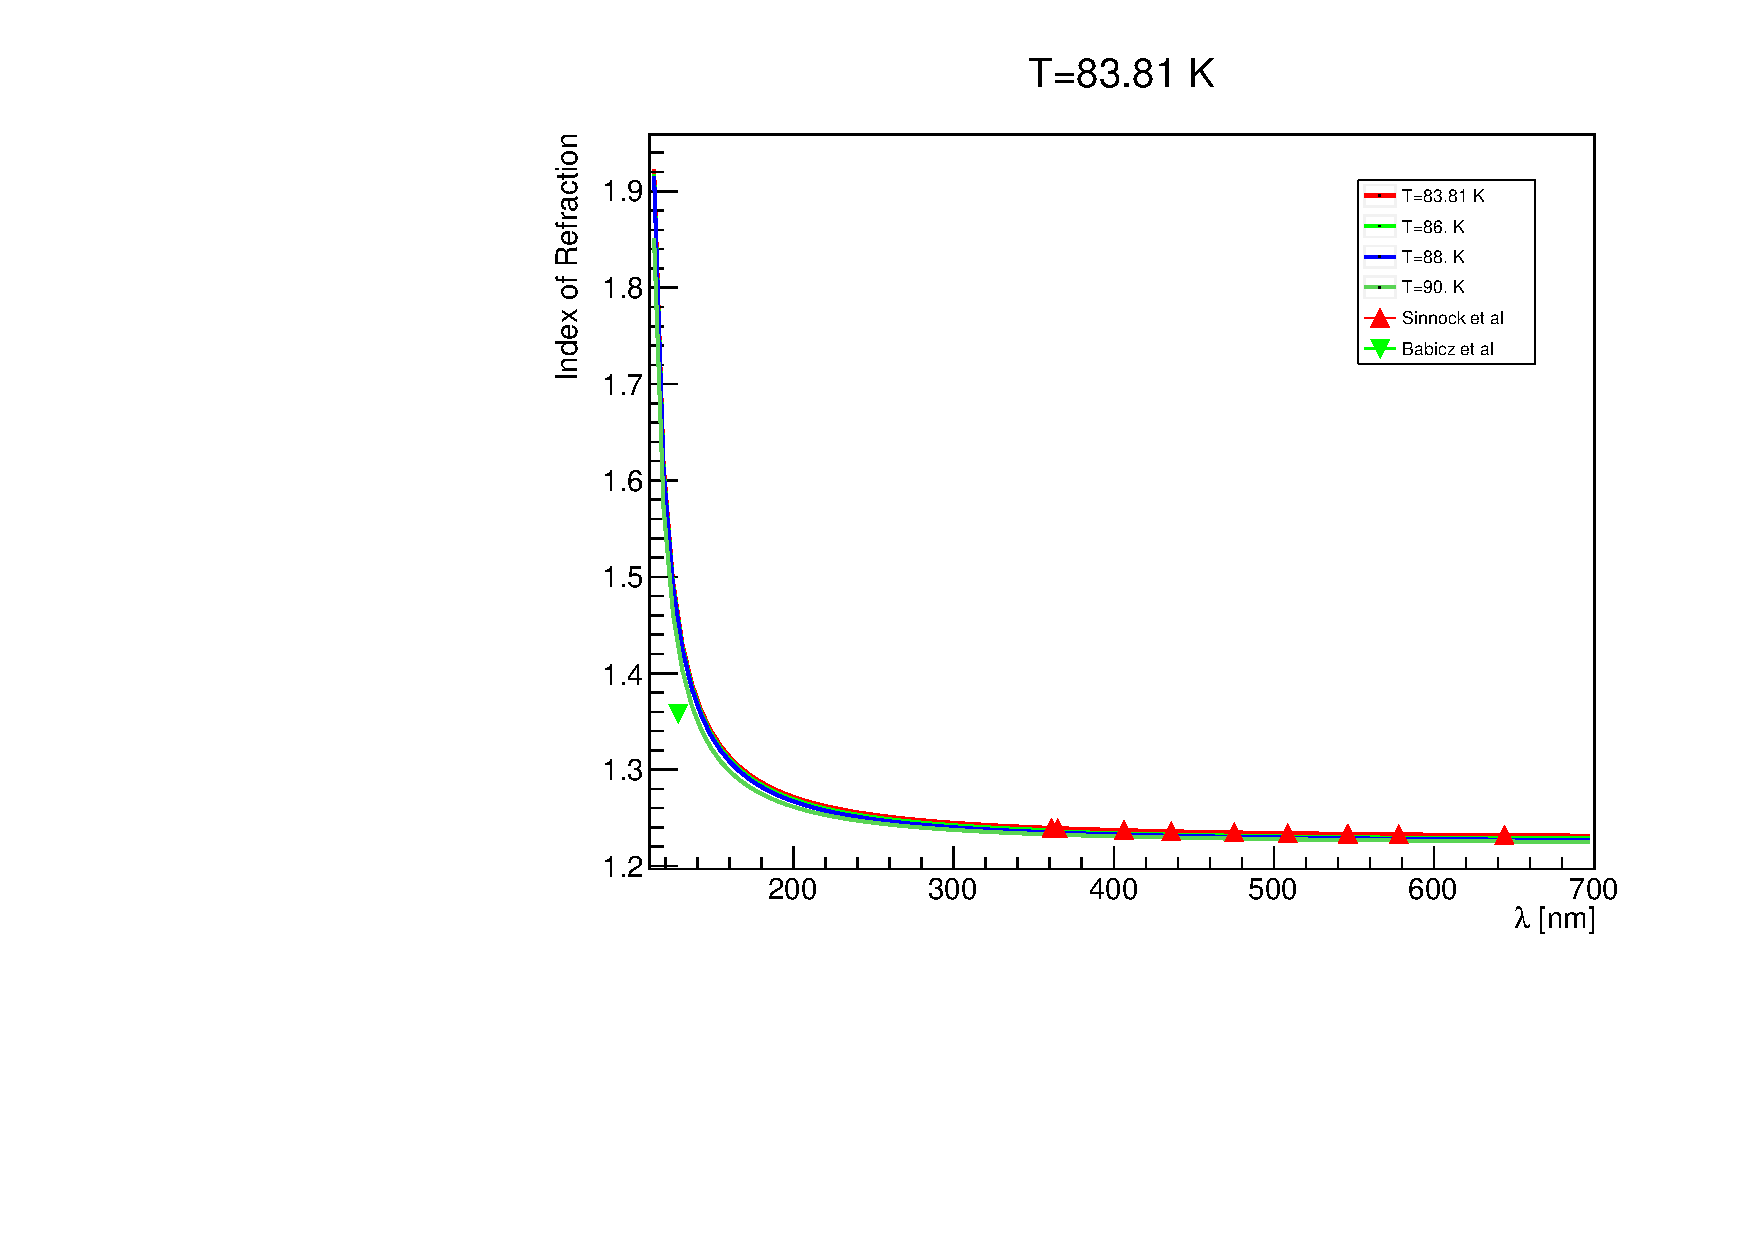
\includegraphics[width=35.5pc]{sellmeier.pdf}
\end{center}
\caption{\label{fig:sellmeier}refraction index}
\end{figure}
\begin{figure}[ht]
\begin{center}
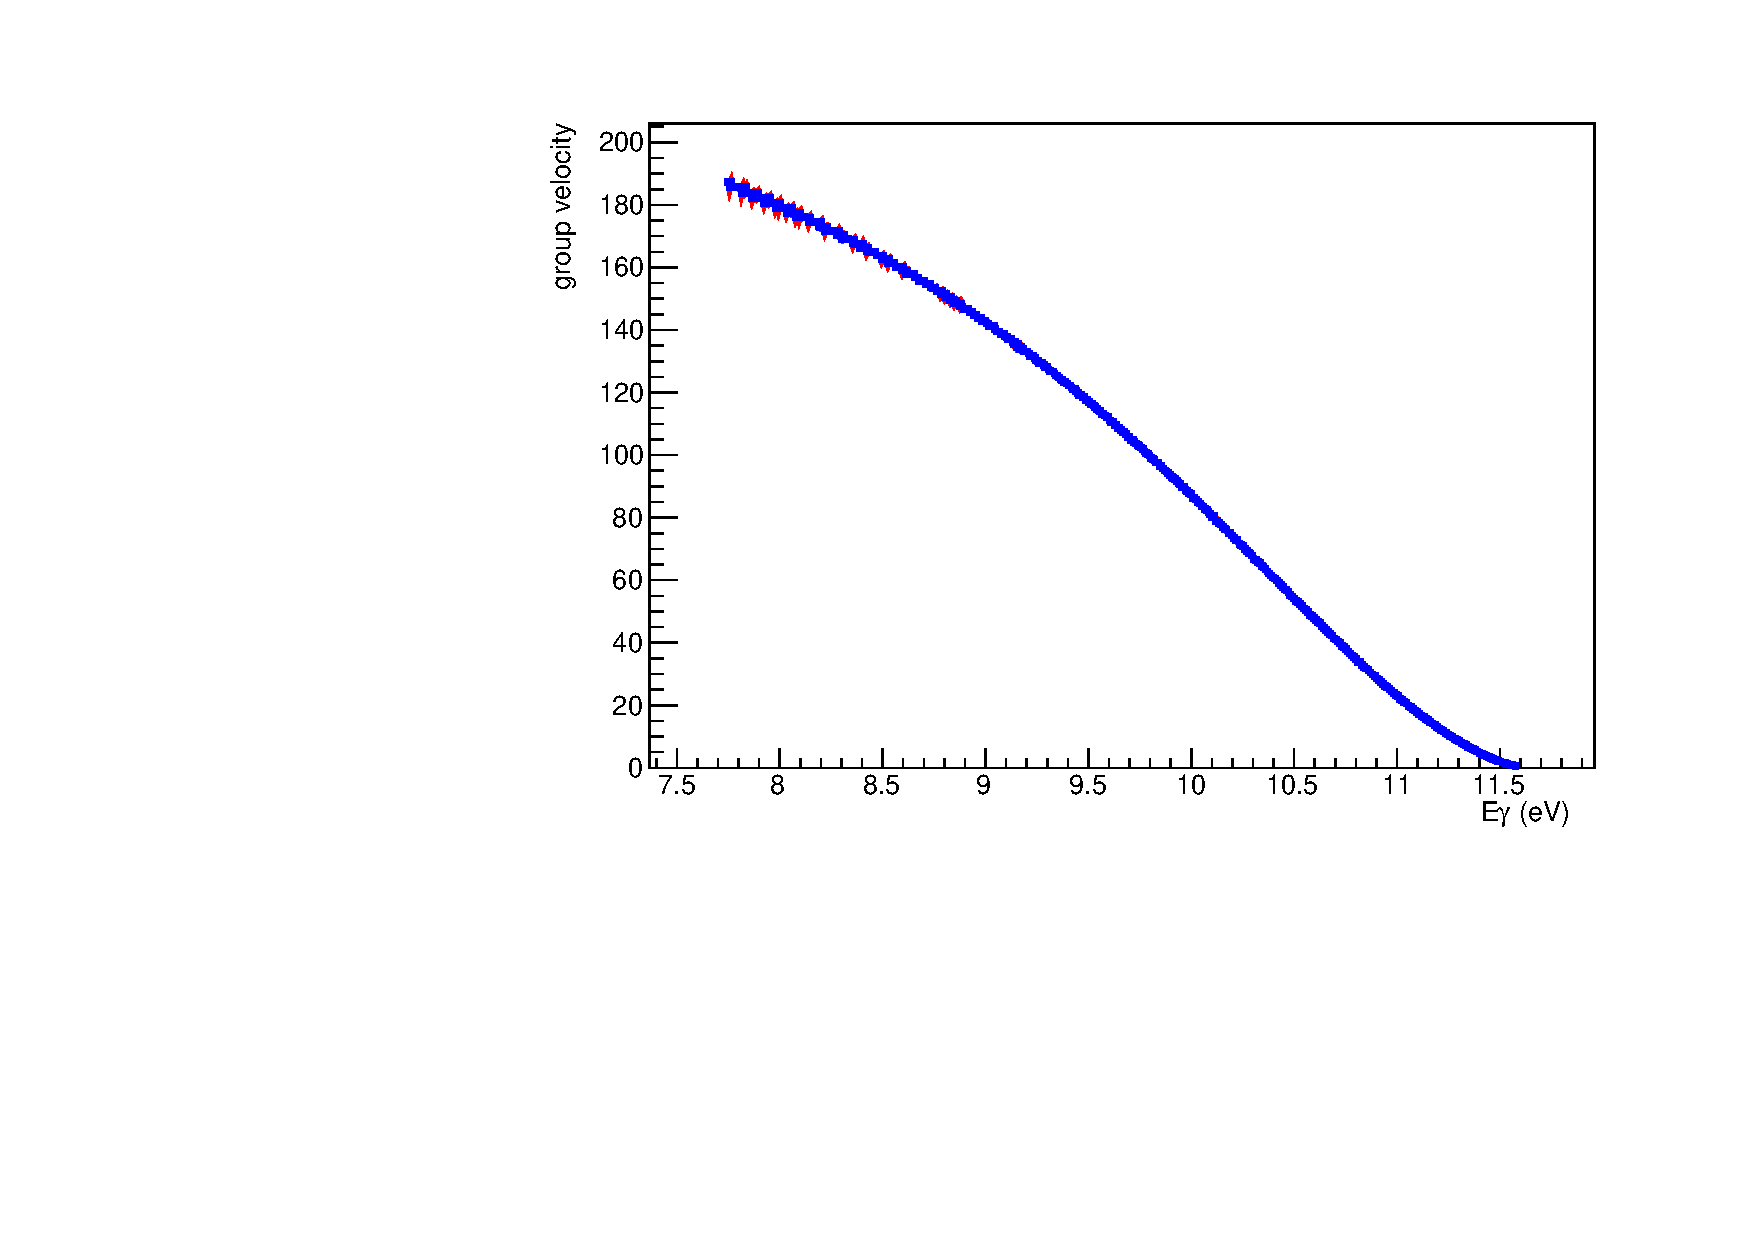
\includegraphics[width=35.5pc]{vg.pdf}
\end{center}
\caption{\label{fig:vg}group velocity}
\end{figure}
\subsection{Absorption length}
Argon is highly transparent to its own scintillation light. (ABSLENGTH)
  $> 1.1 m$  (ArXiv:1511.07725) 
  \subsection{Rayleigh Scattering length}
  Rayleigh scattering length (RAYLEIGH). In the literature one can find the following calculated values at $128 nm$:  90 cm \cite{ref:vg}
  and $55\pm  5 cm$ \cite{ref:grace}. The  range of values for the Rayleigh
scattering length $l$is due to the different refraction indices $n$ at $128nm$  input  to equation  \ref{equ:rayleigh} below:

  \begin{equation}
l^{-1} = \frac{16\pi^3}{6\lambda^4} \left[ kT \rho^2 k_T \left( \frac{(n^2 - 1)(n^2 + 2)}{3} \right)^2\right]
  \label{equ:rayleigh}
\end{equation}
\noindent
    with\\
    $l$: the scattering length\\
    $\lambda$:  the wavelength of light\\
    $n$: the index of refraction corresponding the wavelength of light\\
    $T$: the temperature \\
    $\rho$: the density \\
    $k_T$: the isothermal compressibility\\
    $k$: the Boltzman constant\\

Figure \ref{fig:rayleigh} shows the rayleigh scattering length as a function of $\lambda$ calculated using formula \ref{equ:rayleigh}.

  
  \begin{figure}[ht]
    \begin{center}
      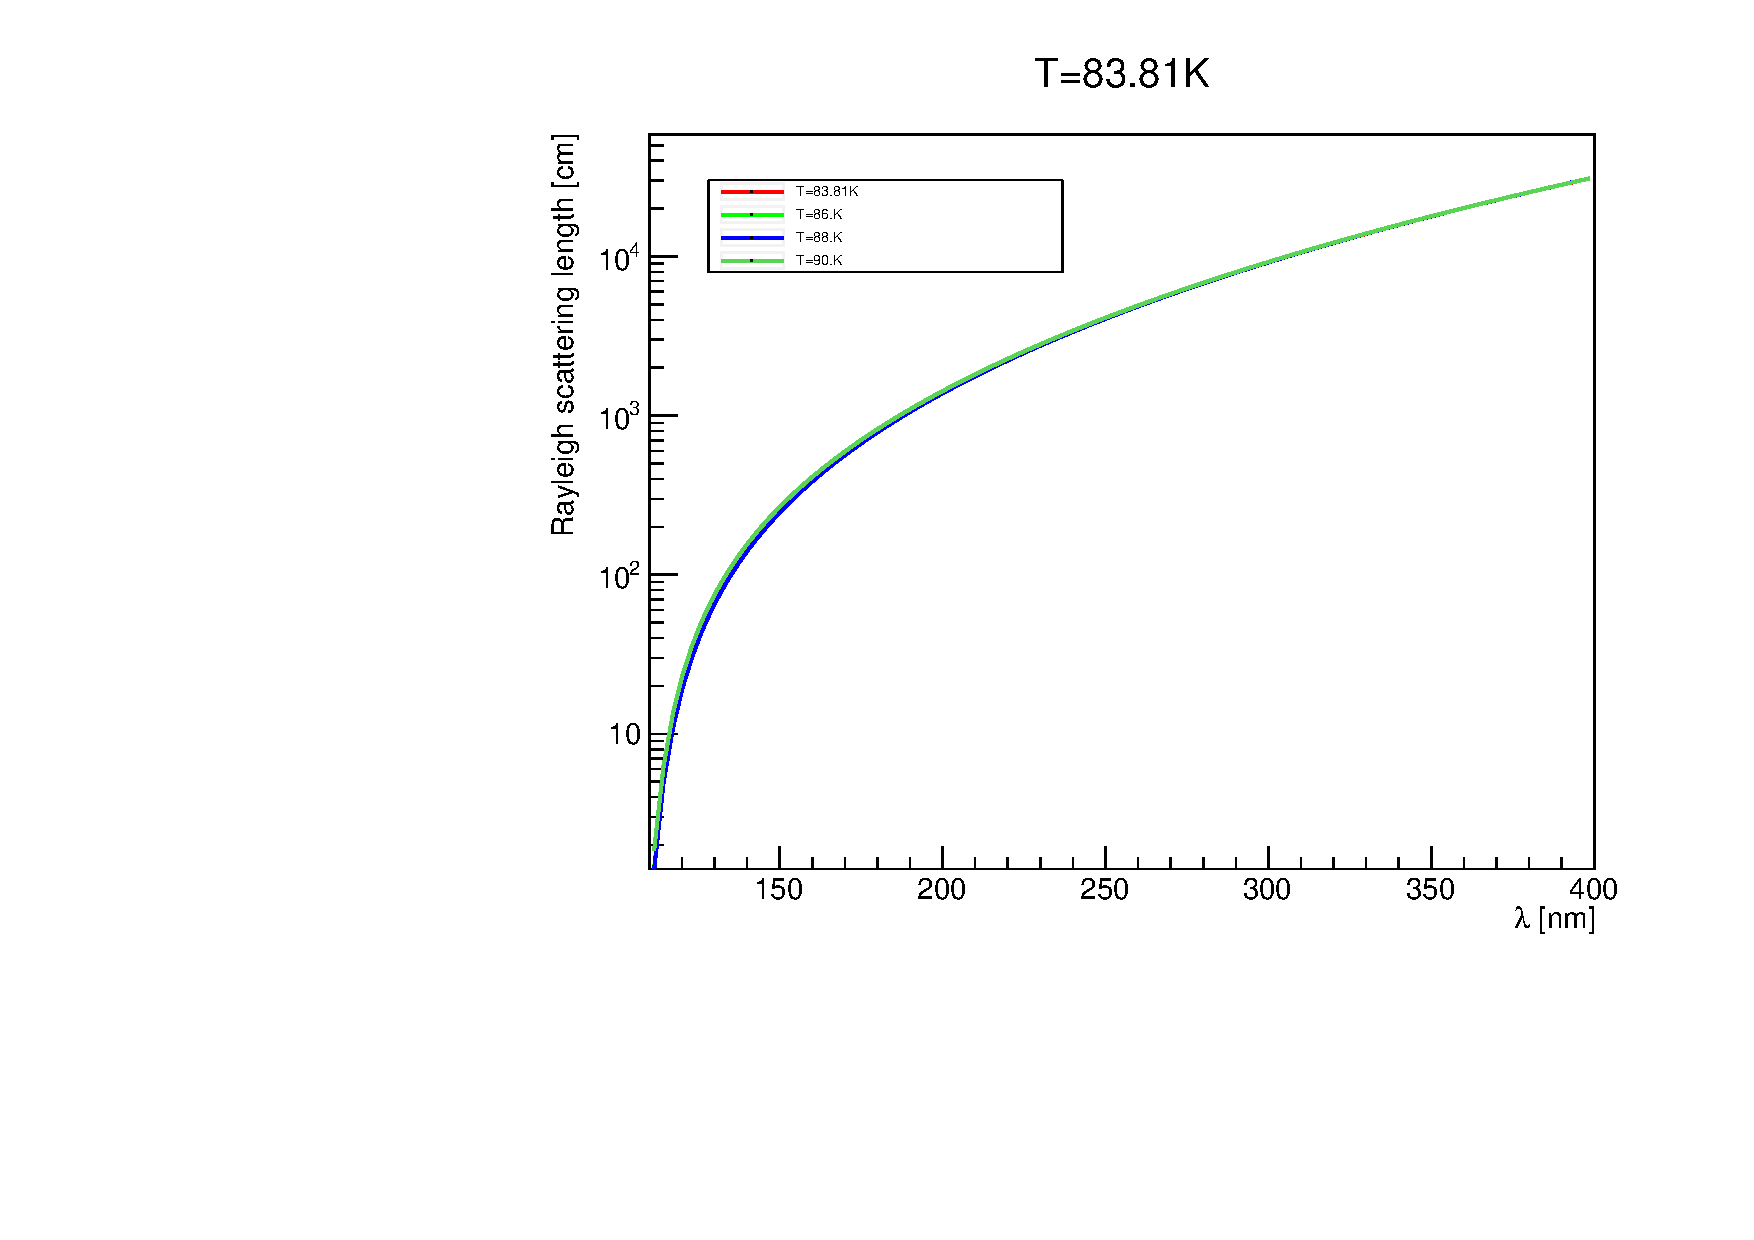
\includegraphics[width=35.5pc]{rayleigh.pdf}
    \end{center}
    \caption{\label{fig:rayleigh}rayleigh scattering length as a function of $\lambda$.}
  \end{figure}
  \section{Boundary processes}
  \subsection{Refraction and total internal reflection}
Refraction is the change in direction of a wave passing from one medium to another or from a gradual change in the medium.
Total internal reflection is the optical phenomenon in which waves arriving at the interface (boundary) from one medium to another (e.g., from water to air) are not refracted into the second ("external") medium, but completely reflected back into the first ("internal") medium. It occurs when the second medium has a higher wave speed (lower refractive index) than the first, and the waves are incident at a sufficiently oblique angle on the interface.
For light, refraction follows Snell's law, which states that, for a given pair of media, the ratio of the sines of the angle of incidence $\theta_1$ and angle of refraction $\theta_2$ is equal to the ratio of phase velocities (v1 / v2) in the two media, or equivalently, to the indices of refraction (n2 / n1) of the two media.

  \begin{equation}
    \frac{\sin \theta _{1}}{\sin \theta _{2}}=\frac{v_{1}}{v_{2}}=\frac {n_{2}}{n_{1}}
  \label{equ:snell}
\end{equation}
    n which waves arriving at the interface (boundary) from one medium to another
  The Fresnel equations (or Fresnel coefficients) describe the reflection and transmission of light (or electromagnetic radiation in general) when incident on an interface between different optical media.(boundary between liquid Ar and wls, wls and
  photo-detector.)

\subsection{reflection} 
 Specular reflection, or regular reflection, is the mirror-like reflection of waves, such as light, from a surface.
  The law of reflection states that a reflected ray of light emerges from the reflecting surface at the same angle to the surface normal as the incident ray, but on the opposing side of the surface normal in the plane formed by the incident and reflected rays.
  (boundary between liquid  Argon and metal walls of cryogenic vessel)



  
  \clearpage
  \section{Photon Detection}
\subsection{Quantum efficiency and absorption length of the tetraphenyl butadiene (TPB) wave length shifter}
\cite{ref:wls}
\begin{table}[h!]
  \begin{center}
    \label{tab:wls}
    \begin{tabular}{|c|c|c|} 
      \hline
      \textbf{optical material property} &\textbf{ Geant4 Keyword} & \textbf{value}\\
      \hline
      Emission spectrum as function of photon energy & WLSCOMPONENT & see Figure \ref{fig:wls} (from  \cite{ref:wls}) \ \\
      Absorption length as function of photon energy & WLSABSLENGTH & $400 nm$ at $128 nm$ \\
      emission time const                           &  WLSTIMECONSTANT        & $0.5 ns$  \\
      \hline
    \end{tabular}
  \end{center}
  \caption{Properties of the TPB wavelength shifter (values from \cite{ref:wls}).}
 \end{table}


\begin{figure}[ht]
\begin{center}
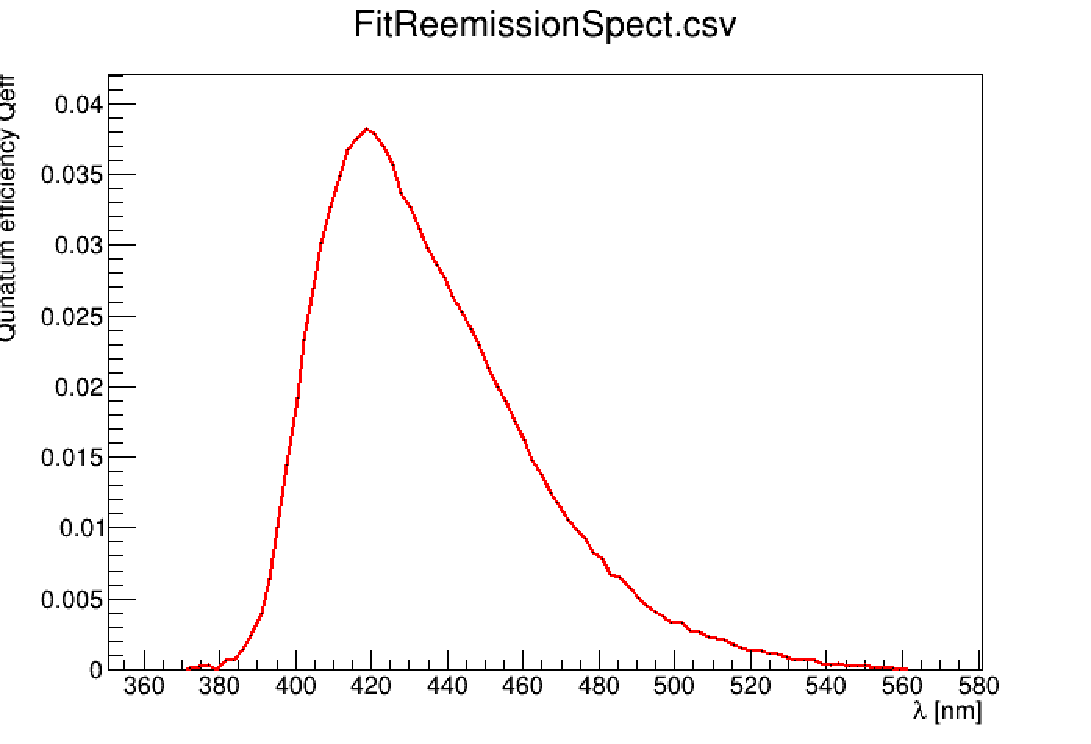
\includegraphics[width=35.5pc]{wls.pdf}
\end{center}
\caption{\label{fig:wls} TPB wave length spectrum extracted from \cite{ref:wls}.}
\end{figure}

\section{Conclusions and Outlook}
\clearpage
 \section*{References}

 \begin{thebibliography}{99}
 \bibitem{ref:LArProperties}
   \verb|https://github.com/hanswenzel/LArProperties|.
 \bibitem{ref:CaTS}
   \verb|https://github.com/hanswenzel/CaTS|.
\bibitem{ref:Geant4-4}
 Allison J et al. 2016, {\it Nuclear Instruments and Methods in Physics
                Research A} {\bf 835} (186--225).
\bibitem{ref:Geant4}
 \verb|http://geant.cern.ch/|.
\bibitem{ref:inspire} High-Energy Physics Literature Database,
  \verb"http://inspirehep.net"/.
\bibitem{ref:scripts}  
  \verb|https://github.com/hanswenzel/CaTS/tree/master/scripts/LAr.C|.\\
  \verb|https://github.com/hanswenzel/CaTS/tree/master/scripts/wls.C|.

\bibitem{ref:wls} Christopher Benson, Gabriel D. Orebi Gann, Victor Gehman,\\
  {\it Measurements of the intrinsic quantum efficiency and absorption
      length of tetraphenyl butadiene thin films in the vacuum
      ultraviolet regime.}\\
Eur. Phys. J. C (2018) 78:329
\bibitem{ref:grace}Emily Grace, Alistair Butcher, Jocelyn Monroe, James A. Nikkel,\\
  \it{Index of refraction, Rayleigh scattering length, and Sellmeier coefficients in solid and liquid argon and xenon.}\\
  \verb|ArXiv:1502.04213|
\bibitem{ref:vg} 
  \it{A measurement of the group velocity of scintillation light in liquid argon},
  M. Babicz et al, 2020 JINST 15 P09009
\bibitem{ref:ben}
  Ben Jones, \it{Introduction to Scintillation Light in Liquid Argon}
  \verb|http://microboone-exp.fnal.gov|
  \bibitem{morikawa}E. Morikawa, R. Reininger, P. Gürtler, V. Saile, and P. Laporte,\\
\it{Argon, krypton, and xenon excimer luminescence: From the dilute gas to the
condensed phase.}\\
J. Chem. Phys. 91, 1469 (1989);
  \verb|https://doi.org/10.1063/1.457108|
\bibitem{ref:pdg}
P.A. Zyla et al. (Particle Data Group), Prog. Theor. Exp. Phys. 2020, 083C01 (2020) and 2021 update.
\verb|https://pdg.lbl.gov/|.
\bibitem{ref:wikipedia}
  \verb|https://en.wikipedia.org/wiki/Cherenkov_radiation|
\bibitem{ref:nest}
  \verb|https://nest.physics.ucdavis.edu/|.
\end{thebibliography}

\end{document}
